\section{Introduction}


\begin{figure}[h]
  \centering
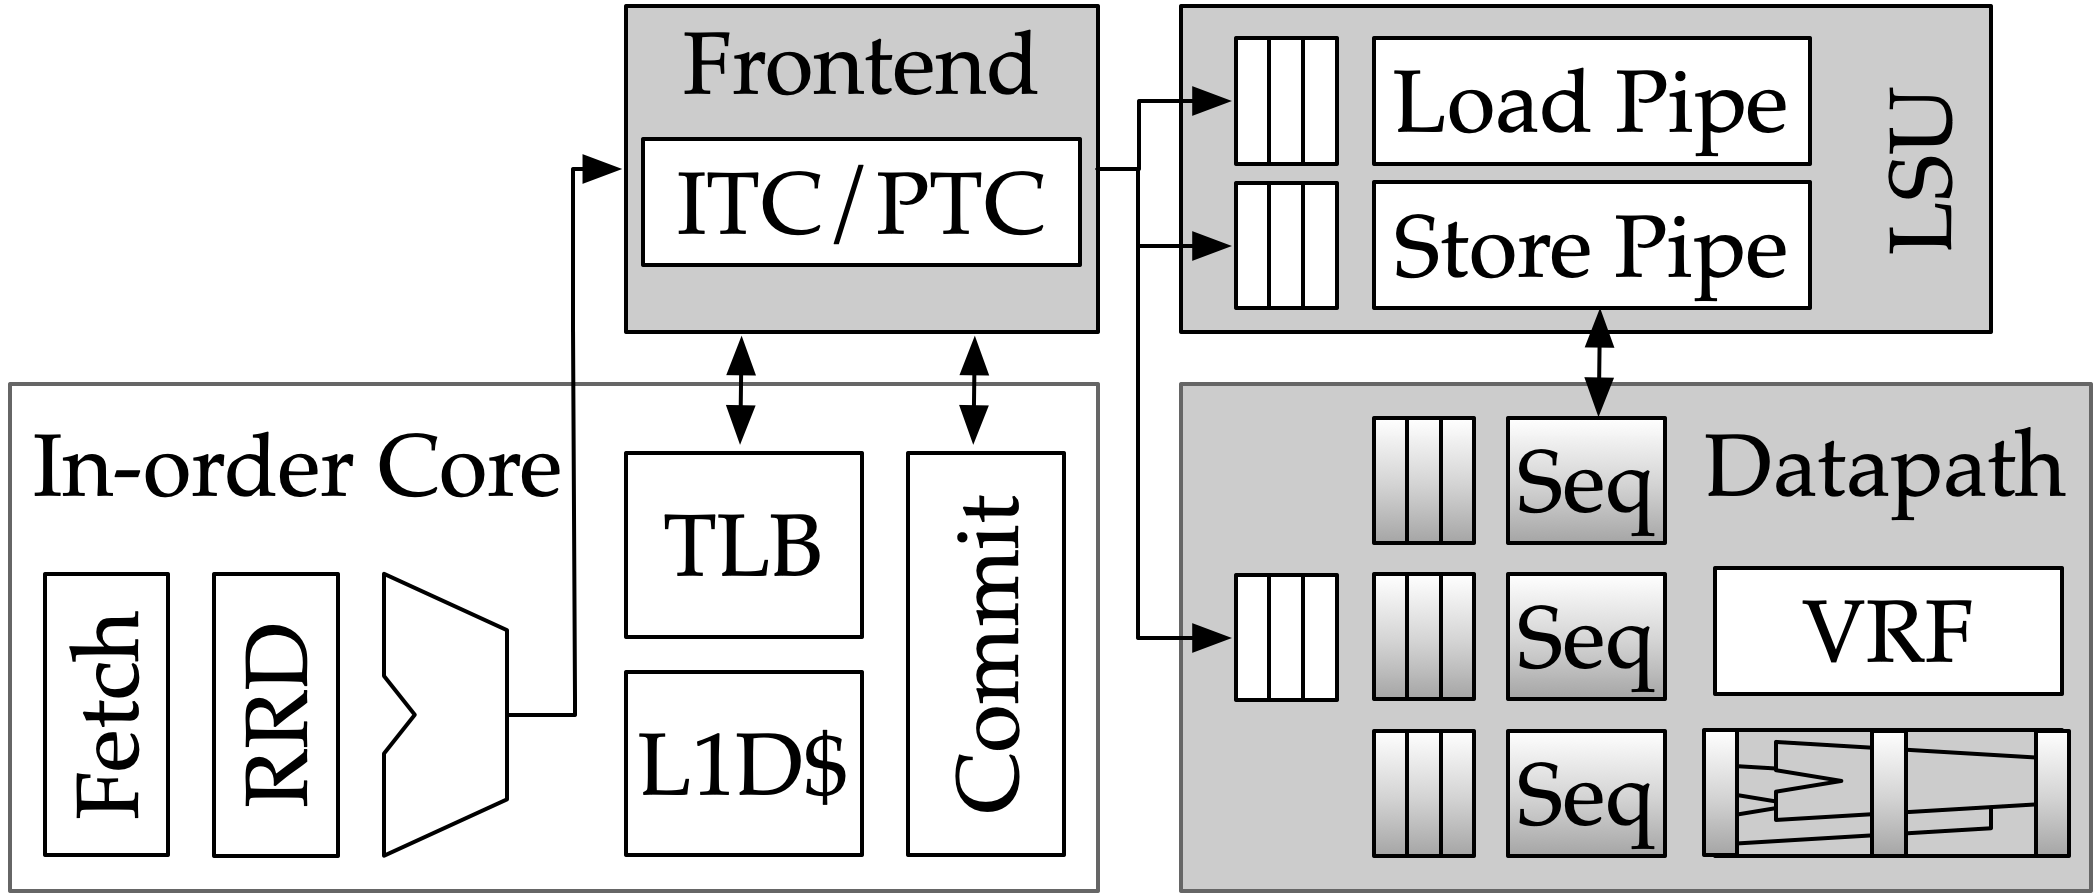
\includegraphics{overview.png}
\caption{A high-level overview of the Saturn Vector Unit}
\end{figure}

This manual describes the Saturn Vector Unit, a parameterized and extensible vector microarchitecture executing the RISC-V vector extension.
Saturn was developed to address an academic need for a representative, compliant, and flexible generator of RISC-V vector units targeting deployment in domain-specialized cores.
Saturn is implemented as a parameterized Chisel RTL generator, enabling a range of possible Saturn configurations across many target deployment scenarios.
This document discusses the microarchitectural details of all Saturn components.

\begin{itemize}
\item Section \ref{sec:background} describes the motivation for Saturn and compares Saturn's design approach to those of existing data-parallel microarchitecture archetypes
\item Section \ref{sec:system} discusses the system organization of Saturn
\item Section \ref{sec:frontend} describes the microarchitecture of Saturn's vector frontend unit
\item Section \ref{sec:memory} describes the microarchitecture of Saturn's vector load-store unit
\item Section \ref{sec:execute} describes the microarchitecture of Saturn's datapath and vector instruction sequencers
\item Section \ref{sec:programming} provides guidance on writing efficient vector code for Saturn
\item Section \ref{sec:history} discusses the historical context of Saturn within past academic vector units
\end{itemize}

\newpage
\subsection{Objectives}

Saturn was developed with the following objectives:

\begin{itemize}
\item Provide a \textbf{representative baseline} implementation of the RISC-V Vector specification
\item Support \textbf{full compliance} with the complete RVV specification, including support for virtual memory and precise faults
\item Target \textbf{ASIC implementations}, rather than FPGA deployments
\item Be sufficiently \textbf{parameterized} to support configurations across a wide power/performance/area design space
\item Demonstrate efficient scheduling of vector operations on a microarchitecture with a \textbf{short hardware vector length}
\item Implement a \textbf{SIMD-style} microarchitecture, comparable to existing SIMD datapaths in DSP microarchitectures
\item Integrate with existing \textbf{efficient area-compact scalar cores}, rather than high-IPC general-purpose cores
\item Support \textbf{extensibility} with custom vector instructions, functional units, and accelerators that leverage the baseline capability in the standard RVV ISA
\item Target deployment as part of a \textbf{DSP core} or similarly domain-specialized core, instead of general-purpose systems
\end{itemize}
